%-------------------------------------------------------------------------------
\section{Validation}\label{sec:evaluation}
%-------------------------------------------------------------------------------
\begin{table}
\caption[]{Description of test sky spectra}
\label{tab:sample}
\centering
\vspace{5pt}
\begin{tabular}{l l c c c c c c}
\hline\hline
\noalign{\smallskip}
label & Instrument & Resol.$^\mathrm{a}$ & $\lambda$ range & Date & Time &
$S_{10.7\,cm}$$^\mathrm{b}$ & Elevation \\
& & & [$\mu$m] & & [UT] & [sfu] & [deg] \\
\noalign{\smallskip}
\hline
\noalign{\smallskip}
fors\_0114 & FORS\,1 & 1200 & $0.54 - 0.75$ & 2000-06-25 & 01:23 & 180 & 54.6\\
fors\_0150 & FORS\,1 & 500 & $0.36 - 0.89$ & 2000-08-26 & 05:48 & 164 & 70.7 \\
fors\_0918 & FORS\,1 & 500 & $0.36 - 0.89$ & 2004-02-26 & 06:23 & 107 & 67.7 \\
fors\_0919 & FORS\,1 & 500 & $0.36 - 0.89$ & 2004-02-26 & 06:59 & 107 & 74.3 \\
fors\_1153 & FORS\,1 & 1200 & $0.54 - 0.75$ & 2004-11-18 & 07:05 & 116 & 55.7\\
fors\_1154 & FORS\,1 & 1200 & $0.54 - 0.75$ & 2004-11-18 & 08:08 & 116 & 46.3\\
sinfo\_1 & SINFONI & 2700 & $1.44 - 1.83$ & 2005-04-03 & 00:00 & 86 & 50.6 \\
sinfo\_2 & SINFONI & 2700 & $1.44 - 1.83$ & 2005-04-03 & 06:32 & 86 & 75.8 \\
sinfo\_4 & SINFONI & 3400 & $1.94 - 2.45$ & 2005-04-03 & 10:05 & 86 & 57.1 \\
sinfo\_5 & SINFONI & 3400 & $1.94 - 2.45$ & 2005-08-11 & 00:54 & 98 & 60.6 \\
sinfo\_6 & SINFONI & 2000 & $1.10 - 1.36$ & 2005-10-31 & 00:34 & 77 & 51.7 \\
sinfo\_7 & SINFONI & 2000 & $1.10 - 1.36$ & 2006-03-13 & 06:05 & 76 & 68.4 \\
xshoo\_28 & X-Shooter & 5300 & $0.99 - 2.00$ & 2010-03-05 & 02:02 & 83 & 55.8\\
xshoo\_29 & X-Shooter & 5300 & $0.99 - 2.00$ & 2010-03-06 & 00:52 & 83 & 57.2\\
xshoo\_39 & X-Shooter & 3200 & $0.99 - 2.00$ & 2010-03-22 & 04:04 & 83 & 64.9\\
xshoo\_42 & X-Shooter & 5300 & $0.99 - 2.00$ & 2010-03-29 & 05:38 & 83 & 56.9\\
xshoo\_43 & X-Shooter & 3200 & $0.99 - 2.00$ & 2010-04-19 & 00:07 & 76 & 42.8\\
xshoo\_44 & X-Shooter & 3200 & $0.99 - 2.00$ & 2010-04-19 & 01:59 & 76 & 62.9\\
\noalign{\smallskip}
\hline
\end{tabular}
\footnotesize
\begin{list}{}{}
\item[$^\mathrm{a}$] mean wavelength / line FWHM
\item[$^\mathrm{b}$] monthly average of solar radio flux at 10.7\,cm in s.f.u.
($= 0.01$\,MJy)
\end{list}
\end{table}

\begin{table}
\caption[]{Test results for pure sky spectra}
\label{tab:results_sky}
\centering
\vspace{5pt}
\footnotesize
\begin{tabular}{l l c c c c c c c c c}
\hline\hline
\noalign{\smallskip}
Target sky & Ref. sky & $N_\mathrm{A}$$^\mathrm{a}$ & $c_\mathrm{A}$$^\mathrm{b}$ &
$N_\mathrm{B}$$^\mathrm{a}$ & $c_\mathrm{B}$$^\mathrm{b}$ & $N_\mathrm{w}$$^\mathrm{a}$ &
$\frac{\sigma(\Delta f_\mathrm{peak})}
{\langle f_\mathrm{peak} \rangle}$$^\mathrm{c}$ &
$\langle \frac{\Delta f_\mathrm{peak}}{f_\mathrm{peak}} \rangle$$^\mathrm{d}$ &
$t_\mathrm{fit}$$^\mathrm{e}$ & $t_\mathrm{code}$$^\mathrm{e}$ \\
& & & & & & & [\%] & [\%] & [s] & [s] \\
\noalign{\smallskip}
\hline
\noalign{\smallskip}
fors\_0918 & fors\_0919 & 13 & $1.00-1.21$ & 10 & $0.98-1.01$ & 6 &
0.3 & 0.3 & 5.1 & 8.7 \\
fors\_0150 & fors\_0919 & 13 & $0.82-1.47$ & 10 & $0.95-1.05$ & 4 &
2.5 & 1.9 & 6.0 & 10.0 \\
fors\_1153 & fors\_1154 & 9 & $0.86-1.00$ & 10 & $0.98-1.00$ & 2 &
0.9 & 0.9 & 2.3 & 5.1 \\
fors\_0114 & fors\_1154 & 9 & $0.70-2.56$ & 10 & $0.52-0.61$ & 8 &
8.6 & 4.3 & 17.6 & 20.0 \\
sinfo\_1 & sinfo\_2 & 6 & $1.84-4.26$ & 14 & $1.12-2.46$ & 4 &
3.0 & 2.7 & 8.8 & 10.3 \\
sinfo\_4 & sinfo\_5 & 3 & $1.25-1.49$ & 10 & $0.84-0.98$ & 2 &
3.7 & 3.3 & 2.1 & 3.6 \\
sinfo\_6 & sinfo\_7 & 5 & $2.00-5.93$ & 16 & $0.88-1.80$ & 4 &
3.6 & 2.9 & 4.4 & 5.9 \\
xshoo\_28 & xshoo\_29 & 17 & $0.37-0.72$ & 20 & $0.93-1.21$ & 5 &
7.3 & 5.8 & 57.3 & 75.8 \\
xshoo\_42 & xshoo\_29 & 17 & $0.18-0.95$ & 20 & $0.52-1.81$ & 3 &
6.5 & 6.9 & 44.4 & 62.4 \\
xshoo\_43 & xshoo\_44 & 17 & $0.82-1.80$ & 20 & $0.71-1.51$ & 0 &
3.0 & 3.1 & 44.8 & 67.3 \\
xshoo\_39 & xshoo\_44 & 17 & $0.37-1.46$ & 20 & $0.89-1.69$ & 3 &
3.7 & 3.6 & 48.7 & 68.0 \\
\noalign{\smallskip}
\hline
\end{tabular}
\footnotesize
\begin{list}{}{}
\item[$^\mathrm{a}$] number of fitted A groups, B groups, and coefficients for
polynomial wavelength grid correction
\item[$^\mathrm{b}$] range of line flux scaling factors for fitted A and B
groups
\item[$^\mathrm{c}$] RMS from difference between modified sky line peaks and
input science line peaks relative to mean of science line peaks (flag~$\ge 2$;
see Section~\ref{sec:linesearch}). The values can be higher if unclipped object
emission lines contribute to the RMS measurement (see
Section~\ref{sec:linefit}).
\item[$^\mathrm{d}$] $\sigma$-clipped mean ratio of sky correction residual and
line flux for line peaks
\item[$^\mathrm{e}$] tested on a Core2Quad Q9550@2.83GHz, 8GB RAM, Fedora 16
(64 bit)
\end{list}
\end{table}

\begin{table}
\caption[]{Test results for object spectra}
\label{tab:results_obj}
\centering
\vspace{5pt}
\footnotesize
\begin{tabular}{l l l c c c c c c c c c}
\hline\hline
\noalign{\smallskip}
Object$^\mathrm{a}$ & Object sky & Ref. sky & $N_\mathrm{A}$$^\mathrm{b}$ &
$c_\mathrm{A}$$^\mathrm{c}$ & $N_\mathrm{B}$$^\mathrm{b}$ & $c_\mathrm{B}$$^\mathrm{c}$ &
$N_\mathrm{w}$$^\mathrm{b}$ & $\frac{\sigma(\Delta f_\mathrm{peak})}
{\langle f_\mathrm{peak} \rangle}$$^\mathrm{d}$ &
$\langle \frac{\Delta f_\mathrm{peak}}{f_\mathrm{peak}} \rangle$$^\mathrm{e}$ &
$t_\mathrm{fit}$$^\mathrm{f}$ & $t_\mathrm{code}$$^\mathrm{f}$ \\
& & & & & & & & [\%] & [\%] & [s] & [s] \\
\noalign{\smallskip}
\hline
\noalign{\smallskip}
NGC\,4594 & fors\_0918 & fors\_0919 & 13 & $0.88-2.78$ & 10 & $0.61-0.97$ & 4 &
9.2 & 12.1 & 5.2 & 8.8 \\
NGC\,4625 & fors\_0918 & fors\_0919 & 12 & $0.29-1.58$ & 10 & $0.81-1.44$ & 0 &
21.6 & 18.8 & 11.0 & 14.9 \\
NGC\,4594 & sinfo\_1 & sinfo\_2 & 6 & $2.09-7.48$ & 10 & $1.05-1.16$ & 0 &
3.5 & 3.3 & 4.0 & 6.3 \\
NGC\,4625 & sinfo\_1 & sinfo\_2 & 6 & $1.93-7.73$ & 10 & $1.14-1.27$ & 3 &
3.4 & 2.9 & 2.4 & 4.6 \\
NGC\,4594 & sinfo\_6 & sinfo\_7 & 5 & $1.69-2.58$ & 16 & $1.11-2.39$ & 0 &
17.5 & 16.6 & 11.1 & 13.1 \\
NGC\,4625 & sinfo\_6 & sinfo\_7 & 5 & $1.92-2.93$ & 16 & $1.08-2.23$ & 0 &
23.2 & 16.2 & 6.3 & 8.0 \\
NGC\,4594 & xshoo\_28 & xshoo\_29 & 16 & $0.40-0.75$ & 16 & $0.95-1.19$ & 7 &
6.9 & 5.6 & 75.3 & 96.9 \\
NGC\,4625 & xshoo\_28 & xshoo\_29 & 16 & $0.41-0.75$ & 16 & $0.86-1.10$ & 5 &
6.6 & 5.5 & 54.2 & 76.1 \\
NGC\,4594 & xshoo\_43 & xshoo\_44 & 17 & $0.77-1.21$ & 16 & $1.00-2.11$ & 0 &
3.5 & 3.8 & 51.6 & 78.2 \\
NGC\,4625 & xshoo\_43 & xshoo\_44 & 17 & $0.61-2.16$ & 10 & $0.97-1.10$ & 0 &
3.5 & 3.8 & 26.1 & 48.8 \\
\noalign{\smallskip}
\hline
\end{tabular}
\footnotesize
\begin{list}{}{}
\item[$^\mathrm{a}$] best-fit CIGALE spectrum of given galaxy at $z = 0.5$ with
arbitrary scaling plus additional emission lines at 0.5, 0.61, 0.71, 0.799553,
0.843248, 1.12, 1.153871, 1.19, 1.212263, 1.34, 1.50, 1.60, 1.670881, 1.700843,
and 1.77\,$\mu$m depending on the wavelength range of the spectrum
\item[$^\mathrm{b}$] number of fitted A groups, B groups, and coefficients for
polynomial wavelength grid correction
\item[$^\mathrm{c}$] range of line flux scaling factors for fitted A and B
groups
\item[$^\mathrm{d}$] RMS from difference between modified sky line peaks and
input science line peaks relative to mean of science line peaks (flag~$\ge 2$;
see Section~\ref{sec:linesearch}). The values can be higher if unclipped object
emission lines contribute to the RMS measurement (see
Section~\ref{sec:linefit}).
\item[$^\mathrm{e}$] $\sigma$-clipped mean ratio of sky correction residual and
line flux for line peaks
\item[$^\mathrm{f}$] tested on a Core2Quad Q9550@2.83GHz, 8GB RAM, Fedora 16
(64 bit)
\end{list}
\end{table}

\begin{figure}
\centering
\includegraphics[width=0.7\textwidth,clip=true]{figures/TEST-FORS-1_fit.pdf}
\caption[]{Comparison of fors\_0918 (black) and best-fit fors\_0919 (red). The
upper panel shows the input and the best-fit spectra, the lower panel the
residual in two different scalings (black~=~original scaling, green~=~optimal
scaling).}
\label{fig:fors_1}
\end{figure}

\begin{figure}
\centering
\includegraphics[width=0.7\textwidth,clip=true]{figures/TEST-FORS-4_fit.pdf}
\caption[]{Comparison of fors\_0114 (black) and best-fit fors\_1154 (red). The
upper panel shows the input and the best-fit spectra, the lower panel the
residual in two different scalings (black~=~original scaling, green~=~optimal
scaling).}
\label{fig:fors_4}
\end{figure}

\begin{figure}
\centering
\includegraphics[width=0.7\textwidth,clip=true]{figures/TEST-SINFO-J_fit.pdf}
\caption[]{Comparison of sinfo\_6 (black) and best-fit sinfo\_7 (red). The
upper panel shows the input and the best-fit spectra, the lower panel the
residual in two different scalings (black~=~original scaling, green~=~optimal
scaling).}
\label{fig:sinfo_J}
\end{figure}

\begin{figure}
\centering
\includegraphics[width=0.7\textwidth,clip=true]{figures/TEST-SINFO-H_fit.pdf}
\caption[]{Comparison of sinfo\_1 (black) and best-fit sinfo\_2 (red). The
upper panel shows the input and the best-fit spectra, the lower panel the
residual in two different scalings (black~=~original scaling, green~=~optimal
scaling).}
\label{fig:sinfo_H}
\end{figure}

\begin{figure}
\centering
\includegraphics[width=0.7\textwidth,clip=true]{figures/TEST-SINFO-K_fit.pdf}
\caption[]{Comparison of sinfo\_4 (black) and best-fit sinfo\_5 (red). The
upper panel shows the input and the best-fit spectra, the lower panel the
residual in two different scalings (black~=~original scaling, green~=~optimal
scaling).}
\label{fig:sinfo_K}
\end{figure}

\begin{figure}
\centering
\includegraphics[width=0.7\textwidth,clip=true]{figures/TEST-XSHOO-1_fit.pdf}
\caption[]{Comparison of xshoo\_28 (black) and best-fit xshoo\_29 (red). The
upper panel shows the input and the best-fit spectra, the lower panel the
residual in two different scalings (black~=~original scaling, green~=~optimal
scaling).}
\label{fig:xshoo_1}
\end{figure}

\begin{figure}
\centering
\includegraphics[width=0.7\textwidth,clip=true]
{figures/N4594-FORS_overplot_w_gal.pdf}
\caption[]{Comparison of arbitrarily scaled NGC\,4594 spectrum at $z = 0.5$ +
artificial emission lines of equal intensity at 0.5, 0.61, 0.71, 0.799553,
0.843248\,$\mu$m + fors\_0918 (black) and best-fit fors\_0919 (red). The lower
panel shows the sky subtraction residual (red) and the original, not
sky-affected NGC\,4594 spectrum (black).}
\label{fig:fors_1_n4594}
\end{figure}

\begin{figure}
\centering
\includegraphics[width=0.7\textwidth,clip=true]
{figures/N4625-FORS_overplot_w_gal.pdf}
\caption[]{Comparison of arbitrarily scaled NGC\,4625 spectrum at $z = 0.5$ +
artificial emission lines of equal intensity at 0.5, 0.61, 0.71, 0.799553,
0.843248\,$\mu$m + fors\_0918 (black) and best-fit fors\_0919 (red). The lower
panel shows the sky subtraction residual (red) and the original, not
sky-affected NGC\,4625 spectrum (black).}
\label{fig:fors_1_n4625}
\end{figure}

\begin{figure}
\centering
\includegraphics[width=0.7\textwidth,clip=true]
{figures/N4594-SINFO-J_overplot_w_gal.pdf}
\caption[]{Comparison of arbitrarily scaled NGC\,4594 at $z = 0.5$ + artificial
emission lines of equal intensity at 1.12, 1.153871, 1.19, 1.212263, and
1.34\,$\mu$m + sinfo\_6 (black) and best-fit sinfo\_7 (red). The lower panel
shows the sky subtraction residual (red) and the original, not sky-affected
NGC\,4594 spectrum (black).}
\label{fig:sinfo_J_n4594}
\end{figure}

\begin{figure}
\centering
\includegraphics[width=0.7\textwidth,clip=true]
{figures/N4594-SINFO-H_overplot_w_gal.pdf}
\caption[]{Comparison of arbitrarily scaled NGC\,4594 at $z = 0.5$ + artificial
emission lines of equal intensity at 1.50, 1.60, 1.670881, 1.700843, and
1.77\,$\mu$m + sinfo\_1 (black) and best-fit sinfo\_2 (red). The lower panel
shows the sky subtraction residual (red) and the original, not sky-affected
NGC\,4594 spectrum (black).}
\label{fig:sinfo_H_n4594}
\end{figure}

\begin{figure}
\centering
\includegraphics[width=0.7\textwidth,clip=true]{figures/TEST-FORS-4-NC_fit.pdf}
\caption[]{Comparison of fors\_0114 (black) and best-fit fors\_1154 (red) for
no correction of the wavelength grid by the fit of a Chebyshev polynomial. The
upper panel shows the input and the best-fit spectra, the lower panel the
residual in two different scalings (black~=~original scaling, green~=~optimal
scaling).}
\label{fig:fors_4_nc}
\end{figure}

The performance of SKYCORR is discussed in the following.
Section~\ref{sec:testsetup} describes the test set-up. The results are
discussed in Section~\ref{sec:results}. Finally, SKYCORR is compared to the
SINFONI pipeline procedure based on the Davies method
(Section~\ref{sec:compdavies}). Some test data are available in the code
directory {\tt <INST\_DIR>/examples/} (see
Section~\ref{sec:calling_examples}). This folder also contains a set of
X-Shooter spectra, which is extensively discussed in the project's science
report \cite{SM03SR}.

%-------------------------------------------------------------------------------
\subsection{Test set-up}\label{sec:testsetup}
%-------------------------------------------------------------------------------
SKYCORR was applied to sky spectra taken from the sky model verification data
set (see \cite{SM01} User Manual). Spectra from the FORS\,1, SINFONI, and
X-Shooter instruments were used (see Tables~\ref{tab:sample} and
\ref{tab:results_sky}). Davies' \cite{DAV07} method was developed for SINFONI
IR spectra. The present SINFONI data set comprises two $J$-band, two $H$-band,
and three $K$-band spectra. With these data a single test per band was
performed, using one spectrum as input science spectrum and one as reference
sky spectrum. The available SINFONI spectra are challenging for the sky
subtraction procedure, since the spectra of each band show exceptionally
pronounced differences (see \cite{SM01} User Manual). In addition, the $J$-band
spectra were taken about half a year apart. In order to have more realistic
input spectra, we also facilitate four pairs of X-Shooter NIR arm spectra
obtained with $0.9''$ and $1.5''$ slits, respectively. The two combinations for
each instrumental set-up differ in the time difference of both exposures. Short
time periods are in the order of one hour or one night, while long time spreads
are in the order of one month. For long time differences, the available sample
of X-Shooter spectra in not suitable. Finally, we also tested four pairs of
FORS\,1 sky spectra taken with the 300\,V and the 600\,R grism, respectively
(see Patat \cite{PAT08}). Thus, we can also test our code in the optical regime
and for low resolution. The resolution of the FORS spectra is about 500 and
1200, respectively, compared to values between 2000 and 5300 for the IR
spectra. For each grism, the exposure dates and times of the target spectra
were selected to differ from those of the fixed reference sky spectrum by the
order of one hour and several years, respectively. The very long periods
possible for the comprehensive FORS data set allow us to compare airglow
spectra taken during phases of significantly different solar activity.

Since the task of the sky correction procedure is the subtraction of sky
emission from an object spectrum showing a continuum and possible emission
lines, a test that corrects one sky spectrum to fit another one is
insufficient. Therefore, the sky spectra defined as science input were
manipulated by adding an object spectrum (see Table~\ref{tab:results_obj}). For
this, best-fit spectral energy distributions (SEDs) of the nearby galaxies
NGC\,4594 and NGC\,4625 obtained by means of the galaxy SED-fitting code CIGALE
(see Noll et al. \cite{NOL09}) were used. The spectra of the two NGC galaxies
are very different. While NGC\,4594 shows an early-type spectrum without
significant emission lines, NGC\,4625 is a late-type galaxy with strong
emission lines. In order to move more lines and continuum features into a
wavelength range where airglow is strong, the two galaxy SEDs were shifted
to a redshift of $z = 0.5$. The flux of the object spectra was scaled
arbitrarily. The SEDs were scaled such that they exhibit a similar strength as
the airglow emission lines. Since the CIGALE model spectra were optimised to fit
photometry (see Noll et al. \cite{NOL09}), the resolution of the emission lines
in the NGC\,4625 spectrum is significantly lower than the resolution of our
observed test sky spectra. In order to test the code for object emission lines
having the same resolution as the sky lines (and to compensate for the lack of
galaxy emission lines in the near-IR), we added 15 artificial lines of constant
intensity to the NGC\,4594 and NGC\,4625 spectra. Lines were set at 0.5, 0.61,
0.71, 0.799553, 0.843248, 1.12, 1.153871, 1.19, 1.212263, 1.34, 1.50, 1.60,
1.670881, 1.700843, and 1.77\,$\mu$m. Since the positions of 6 lines coincide
with strong OH lines, the conservation of object line strength by the sky
correction procedure can be investigated. The final object spectra were added
to a representative subsample of the 11 target sky spectra defined as science
input (see Table~\ref{tab:results_sky}), which resulted in $2 \times 5$
different test set-ups with object spectrum (see Table~\ref{tab:results_obj}).

For a better comparison of the results and to check the quality of the sky
subtraction with standard parameters, we used identical input parameter files
differing in the input and output file names and the selection of air or
vacuum wavelengths only. The values of the fixed parameters can be found in the
listing of the example parameter file shown in Section~\ref{sec:paramfile}.
The Tables~\ref{tab:results_sky} and \ref{tab:results_obj} exhibit some results
for each test set-up. First, the number of fit parameters is shown. The number
of relevant A and B line group parameters (see Section~\ref{sec:airglow})
depends on the wavelength range covered by the spectra. Moreover, the rejection
of unreliable lines can cause that line groups are not fittable and have to be
scaled by mean factors (see Section~\ref{sec:linefit}). The number of
coefficents of the Chebyshev polynomial for the wavelength grid correction (see
Section~\ref{sec:wavegrid}) is variable, since an automatic search for the best
degree is set by default (see Section~\ref{sec:paramfile}). Then, the ranges of
fitted line group flux correction factors are shown for the A and B groups.
Note that the correction factors for lines groups of OH and O$_2$ can differ
considerably. On the other hand, the range of scaling factors of groups of the
same system (\eg\ OH) can be significantly less spread than implied by the
interval given in the table. As indicator for the quality of the sky correction
procedure, Table~\ref{tab:results_sky} shows the weighted RMS derived from
the difference between best-fit reference sky and input science line peak flux
(no continuum) relative to the mean line peak flux in the science spectrum.
Values in the order of a few per cent can be considered as good. Moreover, the
mean ratio $\langle \frac{\Delta f_\mathrm{peak}}{f_\mathrm{peak}} \rangle$ of sky
correction residual and line flux for a $\sigma$-clippped selection of fitted
line peaks in the science spectrum is exhibited. This second quality measure
can be compared to the relative RMS values. If it is distinctly lower, the
RMS appears to be dominated by a few very strong residuals, since
$\langle \frac{\Delta f_\mathrm{peak}}{f_\mathrm{peak}} \rangle$ is relatively
insensitive to residuals that are much stronger than the average. For a visual
inspection of the fit quality Figures~\ref{fig:fors_1} to
\ref{fig:sinfo_H_n4594} show several representative comparisons between
best-fit sky and input science spectra. Finally, the results tables present the
execution times of the sky line fit and the entire code for each set-up. For
comparing the execution times, it should be noted that the X-Shooter spectra
used have 16766 pixels, which is about an order of magnitude higher than the
2048, 1741, 1921, and 2041 pixels of the FORS, SINFONI $J$-band, SINFONI
$H$-band, and SINFONI $K$-band spectra, respectively. Moreover, a degree of the
optimal Chebyshev polynomial above the minimum degree of 3 of the iterative
polynomial searching algorithm is related to a relatively long execution time,
since for each additional degree the line fitting procedure has to be repeated
(see Section~\ref{sec:wavegrid}).

%-------------------------------------------------------------------------------
\subsection{Results}\label{sec:results}
%-------------------------------------------------------------------------------
In general, the results of the sky correction procedure are satisfying. If only
the results for sky spectra (without science object) as shown in
Table~\ref{tab:results_sky} and Figures~\ref{fig:fors_1} to \ref{fig:xshoo_1}
are compared, the best fits are obtained for the first and third FORS set-up
for which the tabulated RMS is below 1\%. For these set-ups the time
difference between both exposures is very short, \ie\ in the order of one hour
(see Table~\ref{tab:sample}). However, even for combinations of spectra taken
with several years in between the fits are good. The relatively low
S/N of the X-Shooter spectra prevent better RMS values than those given in
the table. Significant systematic residuals are rare. An example are the
insufficently corrected O\,I multiplets at 777 and 845\,nm of the first FORS
set-up (see Figure~\ref{fig:fors_1}). Usually these ionospheric lines are weak
and difficult to detect among the strong OH lines. However, in the case of the
target sky spectrum, a strong amplification of these lines occurred, which was
much stronger than for the other ionospheric lines that mainly determine the
correction of the A\,3 group (see Table~\ref{tab:Agroups}). Consequently, there
are certain situations which impede a good correction of atomic lines
originating in the thermosphere. However, the potentially affected wavelength
ranges are very narrow. Another wavelength range which is difficult to correct
is at about 1.27\,$\mu$m. Figure~\ref{fig:sinfo_J} indicates conspicuous
residuals there. The reason is the presence of a strong O$_2$ band (see
Figure~\ref{fig:o2a00band}) with many overlapping lines at the resolution of
SINFONI in the $J$-band. Hence, the continuum determination and the line group
flux correction is very difficult in this wavelength range. For the case of the
SINFONI example the correction was particularly challenging, since the
intensities of the O$_2$(a-X)(0-0) band in the two input spectra differ by an
extreme factor of about 7 (see Table~\ref{tab:results_sky}). In contrast, the
O$_2$ band correction worked much better for the X-Shooter spectra. The example
shown in Figure~\ref{fig:xshoo_1} only indicates minor residuals. Reasons for
the improved results are probably the lower correction factors ($< 4$) and
the higher resolution (see Table~\ref{tab:sample}). Finally,
Figure~\ref{fig:sinfo_K} exhibiting the results of the SINFONI $K$-band set-up
shows relatively strong residuals beyond 2.3\,$\mu$m. Sky lines in the
remaining spectrum are corrected very well. The emission lines at long
wavelengths (beyond 2.3\,$\mu$m) cannot be corrected by our sky subtraction
code, since these are caused by thermal emission in the lower atmosphere and
not airglow emission in the upper atmosphere. Consequently, the code does not
scale line fluxes in the thermal IR. Note that a high degree of the Chebyshev
polynomial for the wavelength grid correction could be a problem in this
regime because of the required strong extrapolation. The example in
Figure~\ref{fig:sinfo_K} does not seem to be affected by this issue. However,
it shows that the subtracion of the strong thermal continuum, which is mainly
caused by the telescope main mirror and cannot be fitted, can be a problem if
the mirror temperature changes between the science and sky exposures.

Adding an object to the input science frame --quite expectedly-- usually causes
a decrease in the fit quality (see Table~\ref{tab:results_obj}). Nevertheless,
in general, the resulting sky-subtracted spectra are good. Examples are shown
in Figures~\ref{fig:fors_1_n4594} to \ref{fig:sinfo_H_n4594}. Due to a strong
and complex continuum, it can happen that the line group correction factors
become less reliable if the continuum has to be interpolated over a relatively
wide wavelength range. This appears to be the reason for the relatively poor
correction of the OH(9-4) band in the object FORS spectra shown in
Figure~\ref{fig:fors_1_n4594} and \ref{fig:fors_1_n4625} and the
O$_2$(a-X)(0-0) band in the object SINFONI $J$-band spectra (see
Figure~\ref{fig:sinfo_J_n4594}). The X-Shooter spectra complemented by an
object spectrum are much better corrected in this wavelength regime as a
comparison of Tables~\ref{tab:results_obj} and \ref{tab:results_sky} implies.
Here, the relatively high resolution has probably helped to better constrain
the continuum. Figures~\ref{fig:fors_1_n4594} to \ref{fig:sinfo_H_n4594}
illustrate the efficiency of SKYCORR in conserving the flux of object emission
lines. The relatively broad lines of the galaxy spectra and the 5 narrow
artificial lines (with FWHM matching that of the spectral set-up) are well
conserved. Even lines directly positioned on top of airglow lines are regained
almost perfectly. A requirement for such a good fit is that the object lines
are masked by the $\sigma$-clipping approach described in
Section~\ref{sec:linefit}. At least for the tested spectra the algorithm works
very well.

The repeated fitting of airglow lines for different degrees of the Chebyshev
polynomial for the wavelength grid correction (see Section~\ref{sec:wavegrid})
imposes a penalty on the code execution times. Run times from 4 to 97\,s are
tabulated in Tables~\ref{tab:results_sky} and \ref{tab:results_obj}. Most of
this time is consumed by the iterative line fitting procedure. The code can be
accelerated considerably by setting the parameter {\sc cheby\_max} to -1 (see
Section~\ref{sec:paramfile}). In this case, no wavelength correction is
performed. This may be an option for spectra with very good wavelength
calibration. However, if the wavelengths grids of two spectra indicate
significant deviations, it is much better to perform the default fitting
procedure. This is demonstrated by Figure~\ref{fig:fors_4_nc} which shows the
results of the fourth FORS set-up (see Table~\ref{tab:results_sky}) without any
wavelength correction. Compared to Figure~\ref{fig:fors_4} which exhibits the
sky-subtracted spectrum for the standard run, the residuals in
Figure~\ref{fig:fors_4_nc} are extremely strong. The spectrum fors\_0114, which
was taken about four and a half years before the reference spectrum fors\_1154
does not appear to be well calibrated. For example, the central wavelength of
the O\,I line at 557.7\,nm differs by about half a pixel. In this case a good
wavelength grid correction is mandatory. This result justifies the choice
of {\sc cheby\_max}~=~7 and {\sc cheby\_min}~=~3 for the standard run, which
aims at providing acceptable sky-corrected spectra for all kinds of input data.

%-------------------------------------------------------------------------------
\subsection{Comparison to Davies' code}\label{sec:compdavies}
%-------------------------------------------------------------------------------
For a concluding evaluation of the performance of SKYCORR, it is required to
compare the present results to those of Davies' code, which is part of the
SINFONI data reduction pipeline (see Section~\ref{sec:davies}).

%-------------------------------------------------------------------------------
\subsubsection{Results for the test set-up}\label{sec:restest}
%-------------------------------------------------------------------------------
\begin{table}
\caption[]{Comparison of SKYCORR and Davies' code}
\label{tab:davies}
\centering
\vspace{5pt}
\begin{tabular}{l c c c c}
\hline\hline
\noalign{\smallskip}
Sample$^\mathrm{a}$ &
$\frac{RMS_\mathrm{SKYCORR}}{\langle f_\mathrm{peak} \rangle}$$^\mathrm{b}$ [\%] &
$\frac{RMS_\mathrm{Davies}}{\langle f_\mathrm{peak} \rangle}$$^\mathrm{b}$ [\%] &
$\frac{RMS_\mathrm{SKYCORR}}{RMS_\mathrm{Davies}}$ [\%] &
$\frac{\langle|\Delta|\rangle_\mathrm{SKYCORR}}
{\langle|\Delta|\rangle_\mathrm{Davies}}$$^\mathrm{c}$ [\%] \\
\noalign{\smallskip}
\hline
\noalign{\smallskip}
Pure sky & $3.9 \pm 2.9$ & $9.7 \pm 8.0$ & $47.4 \pm 21.0$ & $41.0 \pm 15.4$ \\
Object + sky & $4.8 \pm 5.3$ & $7.6 \pm 7.8$ & $60.4 \pm \ \, 9.0$ &
$46.1 \pm \ \, 6.2$ \\
All & $4.4 \pm 4.2$ & $8.6 \pm 7.7$ & $54.3 \pm 16.6$ & $43.7 \pm 11.3$ \\
\noalign{\smallskip}
\hline
\end{tabular}
\footnotesize
\begin{list}{}{}
\item[$^\mathrm{a}$] FORS spectra are not considered, since Davies' code cannot
handle wavelengths below 1\,$\mu$m.
\item[$^\mathrm{b}$] RMS (and its scatter) from difference between residual
flux of sky correction by SKYCORR or Davies' code and pure object spectrum
(zero line for pure sky spectra) relative to mean flux of science spectrum line
peaks (flag~$\ge 2$; see Section~\ref{sec:linesearch}). For the RMS, all
pixels are considered except for wavelengths beyond 2.3\,$\mu$m, where emission
from the lower atmosphere dominates the spectra.
\item[$^\mathrm{c}$] Ratio of results of SKYCORR and Davies' code for mean
absolute difference between residual flux of sky correction and pure object
spectrum. Only wavelengths up to 2.3\,$\mu$m are considered.
\end{list}
\end{table}

\begin{figure}
\centering
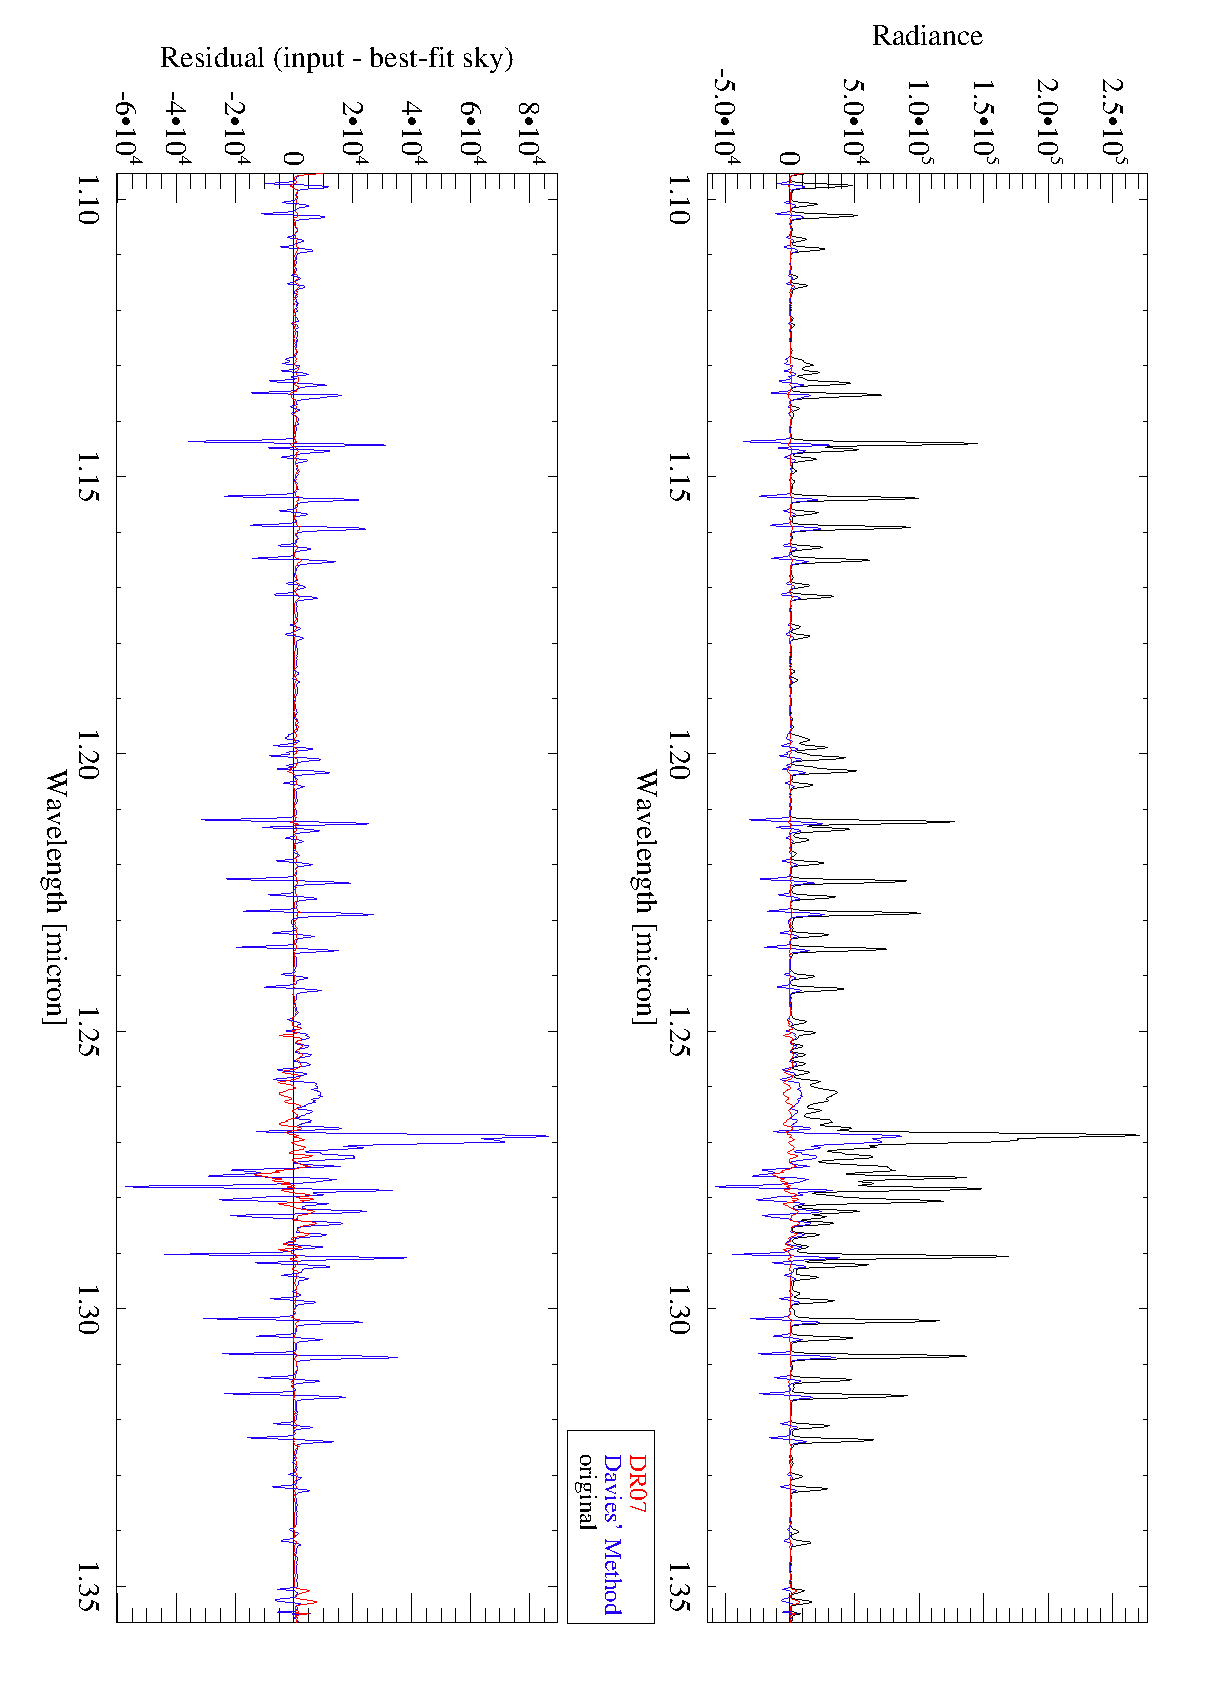
\includegraphics[width=8.8cm,clip=true,angle=90]
{figures/TEST-SINFO-J_comp.eps}
\caption[]{Comparison of SKYCORR (red) and Davies' code results (blue) for the
SINFONI $J$-band set-up without object spectrum (cf. Figure~\ref{fig:sinfo_J}).
Apart from the residuals of the sky correction procedure the upper panel also
shows the input science spectrum (black).}
\label{fig:sinfo_J_comp}
\end{figure}

\begin{figure}
\centering
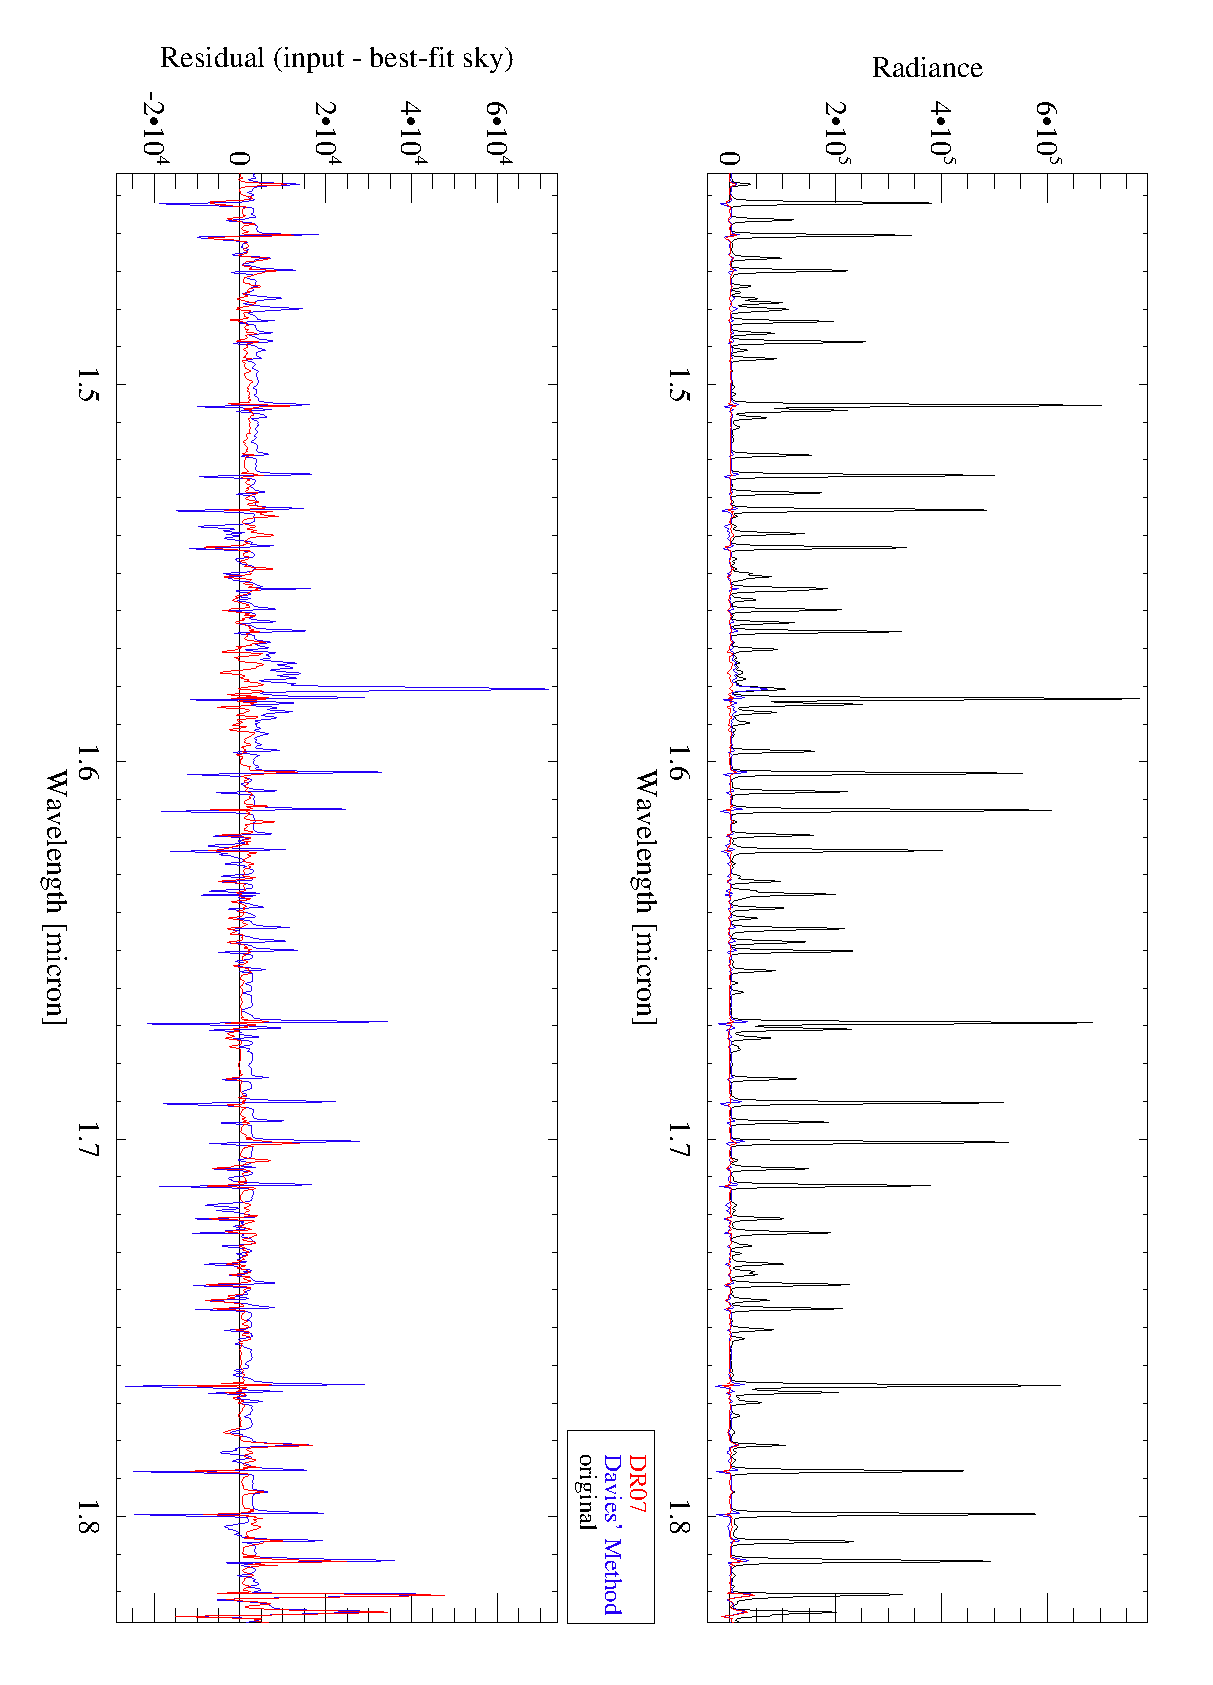
\includegraphics[width=8.8cm,clip=true,angle=90]
{figures/TEST-SINFO-H_comp.eps}
\caption[]{Comparison of SKYCORR (red) and Davies' code results (blue) for the
SINFONI $H$-band set-up without object spectrum (cf. Figure~\ref{fig:sinfo_H}).
Apart from the residuals of the sky correction procedure the upper panel also
shows the input science spectrum (black).}
\label{fig:sinfo_H_comp}
\end{figure}

\begin{figure}
\centering
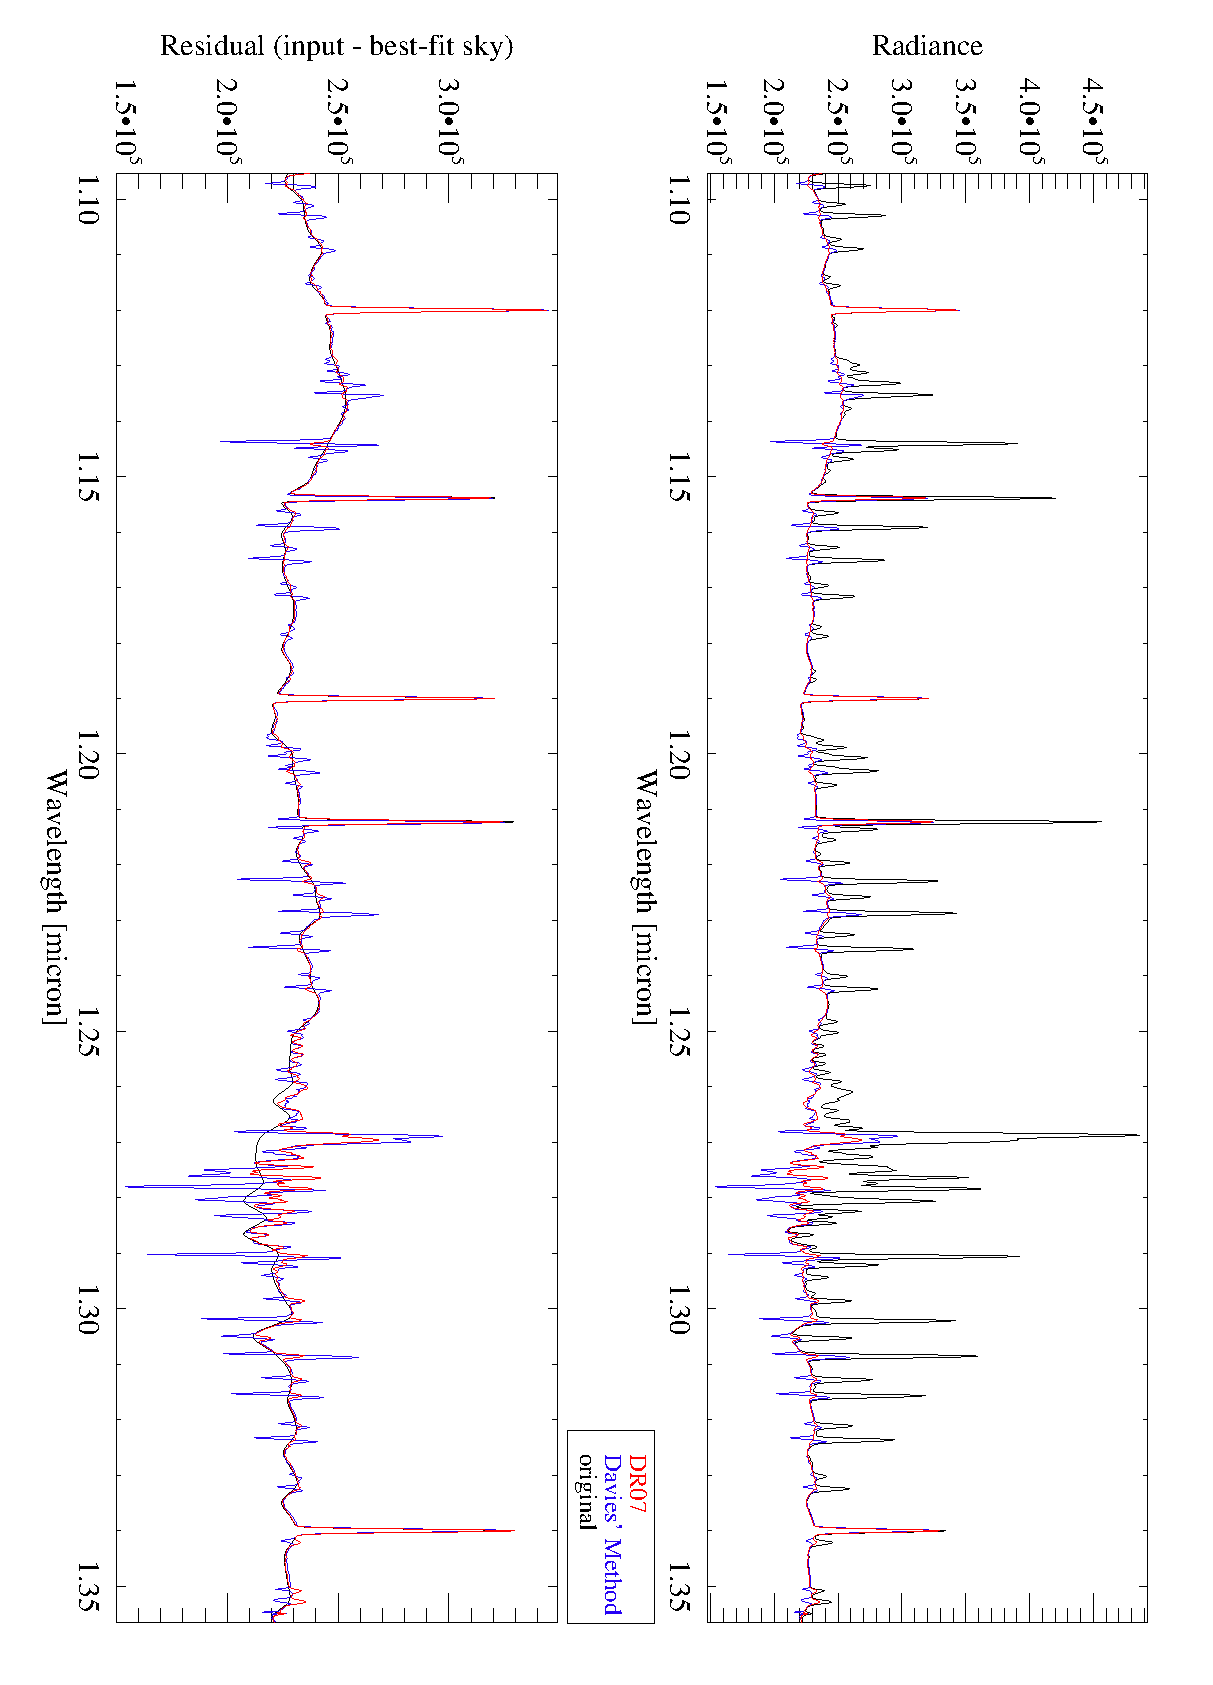
\includegraphics[width=8.8cm,clip=true,angle=90]
{figures/N4594-SINFO-J_comp.eps}
\caption[]{Comparison of SKYCORR (red) and Davies' code results (blue) for the
SINFONI $J$-band set-up with object spectrum (cf.
Figure~\ref{fig:sinfo_J_n4594}). Apart from the residuals of the sky correction
procedure the upper panel also shows the input science spectrum (black).}
\label{fig:sinfo_J_n4594_comp}
\end{figure}

A slightly adapted version of Davies' code was run on our test data set
described in Section~\ref{sec:testsetup}. The FORS set-ups have not been
tested, since Davies' code is not able to correct airglow lines at wavelengths
below 1\,$\mu$m. Consequently, the resulting test data set consists of 7 pure
sky and 8 object + sky set-ups. The results of the runs of both codes are
summarised in Table~\ref{tab:davies}. The listing exhibits the relative RMS
mean values and their scatter for the subsample of pure sky spectra, the
subsample of object spectra, and the total sample of 15 set-ups. In contrast to
Tables~\ref{tab:results_sky} and \ref{tab:results_obj}, the RMS was computed
for all pixels of the spectrum. Moreover, the RMS calculation is related to the
difference between the residual of the sky correction and the input object
spectrum which is a zero line for pure sky spectra. The RMS values of both
codes are provided relative to the mean line peak flux in the input science
spectrum. In order to simplify the comparison of the results of both codes, the
ratio of both RMS values is shown as well. Finally, a corresponding ratio for
the mean absolute difference between sky correction residual and pure object
spectrum is indicated. In comparison to the RMS ratio, the latter quantity is
less sensitive to very strong residuals that affect a few pixels only. For this
reason, a high RMS compared to the mean absolute difference suggests that
strong residuals affect a relatively narrow range of the spectrum only.
Examples for the differences in the results of both codes are presented in
Figures~\ref{fig:sinfo_J_comp} to \ref{fig:sinfo_J_n4594_comp}.

Table~\ref{tab:davies} indicates that SKYCORR has an improved performance in
comparison to Davies' code. In the tested set-ups, the RMS of SKYCORR is
lower. On average the RMS ratio is about 54\%. For pure sky spectra, the
results tend to be better than for science spectra incorporating an object
(47\% versus 60\%). This discrepancy is not observed for the mean absolute
difference, where the results for the two subsamples differ from the mean of
44\% only slightly. The differences in the results for both quantities can be
explained --as already mentioned above-- by the dominance of the contribution
to the RMS by a few residual pixels. Such a situation is shown in
Figure~\ref{fig:sinfo_J_n4594_comp}, which indicates relatively strong
residuals for the O$_2$ band at 1.27\,$\mu$m. Apart from the O$_2$ band, where
both codes are comparable, the SKYCORR performance is superior (by a factor of
2 on average). However, this particular band cannot be corrected very well,
since the density of strong lines is very high requiring interpolation of the
continuum over a relatively wide wavelength range. As already discussed in
context of Figure~\ref{fig:sinfo_J}, the interpolation, the complex object
continuum, and the extreme difference in the properties of the two sky spectra,
prevent a good sky correction in this wavelength range.

%-------------------------------------------------------------------------------
\subsubsection{Results for SINFONI pipeline data}\label{sec:ressinfo}
%-------------------------------------------------------------------------------
\begin{figure}
\centering
\includegraphics[width=0.7\textwidth,clip=true]
{figures/scr_comp_sinfo_H_ex1.pdf}
\caption[]{Comparison of SKYCORR (red) and Davies' code results (cyan) for a
SINFONI $H$-band pipeline product. While the upper panel shows the full input
spectrum of HE\,1216, the lower panel focuses on the sky subtraction results.}
\label{fig:sinfo_H_ex1}
\end{figure}

\begin{figure}
\centering
\includegraphics[width=0.7\textwidth,clip=true]
{figures/scr_comp_sinfo_K_ex1.pdf}
\caption[]{Comparison of SKYCORR (red) and Davies' code results (cyan) for a
SINFONI $K$-band pipeline product. While the upper panel shows the full input
spectrum of NGC\,6240, the lower panel focuses on the sky subtraction results.}
\label{fig:sinfo_K_ex1}
\end{figure}

\begin{figure}
\centering
\includegraphics[width=0.7\textwidth,clip=true]
{figures/scr_comp_sinfo_HK_ex1.pdf}
\caption[]{Comparison of SKYCORR (green/red) and Davies' code results (cyan)
for a SINFONI $HK$-band pipeline product. SKYCORR was run for the default
parameter set (green; see Section~\ref{sec:paramfile}) and an optimised
set-up (red), which only differs from the standard by
{\sc min\_line\_dist}~=~12.5. While the upper panel shows the full input
spectrum of TXS\,0828, the lower panel focuses on the sky subtraction results.}
\label{fig:sinfo_HK_ex1}
\end{figure}

For the code evaluation by means of sky model verification data and simulated
object spectra (see Section~\ref{sec:restest}), Davies' code was modified to
handle data that was not processed with this routine before. In order to get a
better idea how SKYCORR would perform if it was used in the SINFONI pipeline
(Modigliani et al.~\cite{MOD07}) instead of the Davies method, one could also
modify the SINFONI pipeline products to allow an application of SKYCORR. For
this purpose, suitable object and reference sky 1D data derived from SINFONI
data cubes for spectroscopic observations in different bands were provided by
A. Modigliani from ESO.

In Figures~\ref{fig:sinfo_H_ex1} to \ref{fig:sinfo_HK_ex1}, we illustrate the
performance of SKYCORR for this realistic data set comprising observations in
the $H$, $K$, and $HK$-band modes. The results are superb for $H$ and $K$ with
relative residuals of about three orders of magnitude weaker than the original
airglow lines. Moreover, the comparison to the Davies code indicates a
significantly better sky subtraction by SKYCORR, which is in agreement with the
results of Section~\ref{sec:restest}. The results of the $HK$ mode are worse
for both codes with residuals up to several per cent. For the default parameter
set-up, the quality of the SKYCORR sky-subtracted spectrum is relatively
similar to the one produced by Davies' code. However, the wavelength position
and shape of the residuals are very different. As demonstrated by
Figure~\ref{fig:sinfo_HK_ex1}, an optimisation of the SKYCORR input parameter
set can distinctly improve the results. To achieve the convincing sky
subtraction, only the {\sc min\_line\_dist} parameter (see
Section~\ref{sec:params}) was set from 2.5 to 12.5. Likewise, another good
result was obtained by changing {\sc fluxlim} from -1 to 0.08. These changes
affect the line finder (Section~\ref{sec:linesearch}) and the separation of
lines and continuum (Section~\ref{sec:contsub}). This makes sense, since the
resolution of the SINFONI $HK$-band mode is relatively low (about 1500;
cf.~Table~\ref{tab:sample}), which causes enhanced line blending. Hence,
the line detection and continuum separation becomes difficult if pseudo
continua consisting of line blends cover large parts of the investigated
spectrum. In particular, the $H$ band around the O$_2$ band at 1.58\,\mum{}
characterised by a high line density (see Figure~\ref{fig:o2a01band}) appears
to be affected by this issue.

Summarising the evaluation section, we can conclude that the SKYCORR sky
correction code produces convincing results for various kinds of data even if
the time period between the object and reference sky exposures is very long. In
general, the results are better than those produced by Davies' code. In most
cases, good sky subtraction can be achieved with a minimum of interaction. If
this is not sufficient, the user can try to fine-tune the sky subtraction by
varying the procedure's input parameters (see Section~\ref{sec:params}). Also,
this will influence the code run time.
